\section{The MLIR Framework}
\subsection{Overview}
MLIR is an optimizing compiler infrastructure inspired by LLVM~\cite{llvm} with a focus on extensibility and modularity~\cite{mlir}. Its main novelty is the IR supporting a fully extensible set of instructions (called \emph{operations}) and types. Practically, MLIR combines SSA with nested regions, allowing one to express a range of concepts as first-class operations including machine instructions such as floating-point addition, structured control flow such as loops, hardware circuitry~\cite{circt}, and large machine learning graphs. Operations define the runtime semantics of a program and process immutable values. Compile-time information about values is expressed in \emph{types}, and information about operations is expressed in \emph{attributes}. Operations can have attached regions, which in turn contain (basic) blocks of further operations. The generic syntax, accepted by all operations, illustrates the structure of MLIR in Figure~\ref{fig:mlir_syntax}. Additionally, MLIR supports user-defined custom syntax.

\begin{figure}
{
\scriptsize
\begin{lstlisting}[language=llvm,escapeinside=@@, mathescape=true]
%result = "dialect.operation"(%operand, %operand)
          {attribute = #dialect<"value">} ({
// Inside a nested region.
^basic_block(%block_argument: !dialect.type):
  "another.operation"() : () -> ()
}) : (!dialect.type) -> !dialect.result_type
\end{lstlisting}
}
\caption{Generic MLIR syntax for an operation with two operands, one result, one attribute and a single-block region.}
\label{fig:mlir_syntax}
\end{figure}

Attributes, operations, and types are organized in \emph{dialects}, which can be thought of as modular libraries. MLIR provides a handful of dialects that define common operations such as modules, functions, loops, memory or arithmetic instructions, and ubiquitous types such as integers and floats. We discuss the dialects relevant to \tool in the following sections.

\subsection{Affine and MemRef Dialects}\label{sec:affine_memref}

The \emph{Affine} dialect~\cite{mlir_affine} aims at representing \scop's with explicit polyhedral-friendly loop and conditional constructs.
The core of its representation is the following classification of value categories:
\begin{itemize}
    \item \emph{Symbols}---integer values that are known to be loop-invariant but unknown at compile-time, also referred to as program \emph{parameters} in polyhedral literature, typically array dimensions or function arguments. In MLIR, symbols are values defined in the top-level region of an operation with ``affine scope'' semantics, e.g., functions; or array dimensions, constants, and affine map (see below) application results regardless of their definition point.
    \item \emph{Dimensions}---are an extension of symbols that also accepts induction variables of affine loops.
    \item \emph{Non-affine}---any other values.
\end{itemize}
Symbols and dimensions have \icode{index} type, which is a platform-specific integer that fits a pointer (\icode{intptr\_t} in C).

MLIR provides two attributes relevant for the Affine dialect:
\begin{itemize}
\item
\emph{Affine maps} are multi-dimensional (quasi-)linear functions that map a list of dimension and symbol arguments to a list of results.
For example, $(d_0, d_1, d_2, s_0) \rightarrow (d_0 + d_1, s_0 \cdot d_2)$ is a two-dimensional quasi-affine map, which can be expressed
in MLIR as \icode{affine\_map<(d0,d1,d2)[s0] -> (d0+d1, s0*d2)>}.
%The affine map construct does \emph{not} require its arguments to have the symbol and dimension category, only \emph{some} operations in the affine dialect do.
Dimensions (in parentheses on the left) and symbols (in brackets on the left) are separated to allow quasi-linear expressions: symbols are treated as constants, which can therefore be multiplied with dimensions, whereas a product of two dimensions is invalid.
\item
\emph{Integer sets} are collections of integer tuples constrained by conjunctions of (quasi-)linear expressions.
For example, a ``triangular'' set $\{(d_0, d_1) : 0 \leq d_0 < s_0 \land 0 \leq d_1 \leq d_0\}$ is represented as
\icode{affine\_set<(d0,d1)[s0]: (d0 >= 0, s0-d0-1 >= 0, d1 >= 0, d0-d1 >= 0)>}.
\end{itemize}


The Affine dialect makes use of the concepts above to define a set of operations.
An \icode{affine.for} is a ``for'' loop with loop-invariant lower and upper bounds expressed as affine maps with a constant step.
An \icode{affine.parallel} is a ``multifor'' loop nest, iterations of which may be executed concurrently.
Both kinds of loops support reductions via loop-carried values as well as max(min) expression lower(upper) bounds.
%The region is a single block that corresponds to the body of the loop and takes the induction variable as a loop argument.
An \icode{affine.if} is a conditional construct, with an optional \icode{else} region, and a condition defined as inclusion of the given values into an integer set.
Finally, \icode{affine.load} and \icode{affine.store} express memory accesses where the address computation is expressed as an affine map.

\begin{figure}
{
\scriptsize
\begin{lstlisting}[language=llvm, escapeinside=@@, mathescape=true]
%c0 = constant 0 : index
%0 = memref.dim %A, %c0 : memref<?xf32>
%1 = memref.dim %B, %c0 : memref<?xf32>
affine.for %i = 0 to affine_map<()[s0] -> (s0)>()[%0] {
  affine.for %j = 0 to affine_map<()[s0] -> (s0)>()[%1] {
    %2 = affine.load %A[%i] : memref<?xf32>
    %3 = affine.load %B[%j] : memref<?xf32>
    %4 = mulf %2, %3 : f32
    %5 = affine.load %C[%i + %j] : memref<?xf32>
    %6 = addf %4, %5 : f32
    affine.store %6, %C[%i + %j] : memref<?xf32>
  }
}
\end{lstlisting}
}
\vspace{-.5cm}
\caption{Polynomial multiplication in MLIR using Affine and Standard dialects.}
\label{fig:polynomial}
\end{figure}

Figure~\ref{fig:polynomial} illustrates the Affine dialect for a polynomial multiplication, \icode{C[i+j] += A[i] * B[j]}.
This simple example highlights the fact that MLIR supports, and encourages, IRs from different dialects to be used together.

% \begin{figure}
%     \centering
%     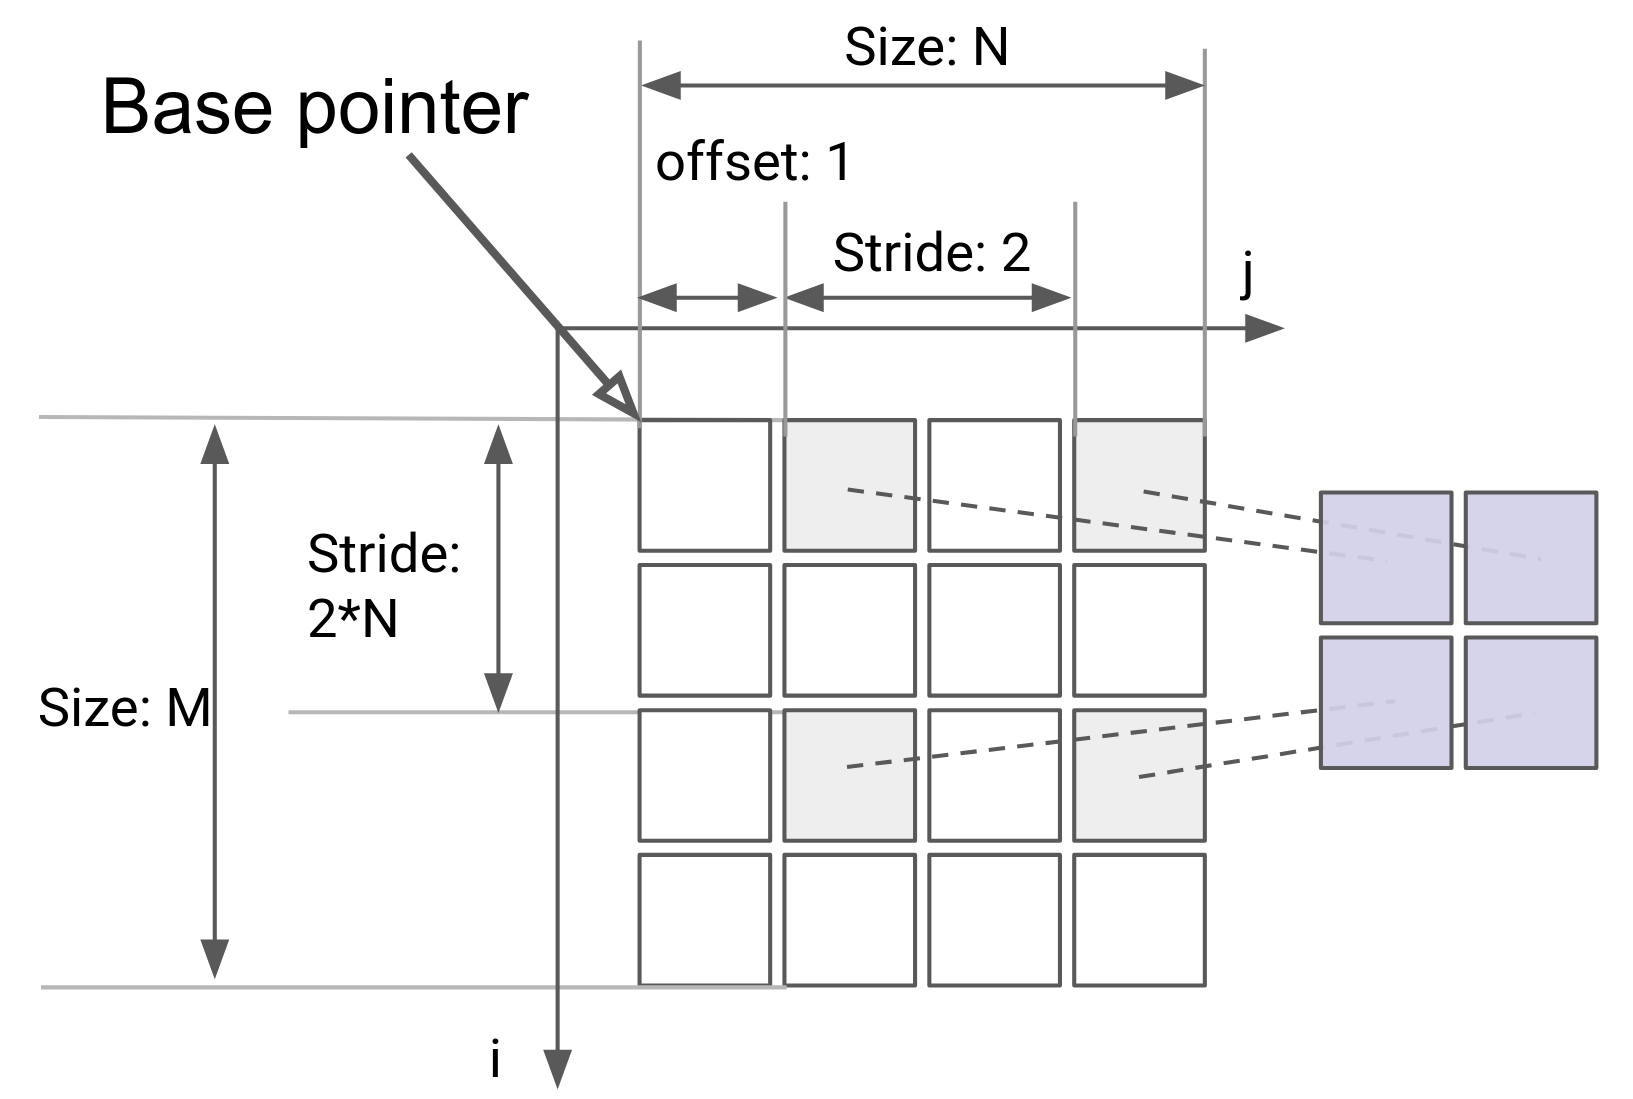
\includegraphics[width=0.7\columnwidth]{images/memref.png}
%     \vspace{-.5cm}
%     \caption{MLIR supports multi-dimensional memory references indexed with affine maps.}
%     \label{fig:memref}
% \end{figure}

A core MLIR type---\memref, which stands for \textbf{mem}ory \textbf{ref}erence---and the corresponding \emph{\memref dialect} are also featured in Figure~\ref{fig:polynomial}. The \memref type describes a structured multi-index pointer into memory, e.g., \icode{memref<?xf32>} denotes a 1-d array of floating-point elements; and the \emph{\memref dialect} provides memory and type manipulation operations, e.g., \icode{memref.dim} retrieves the dimensionality of a \memref object.
\memref does not allow internal aliasing, i.e., different subscripts always point to different addresses.
This effectively defines away the delinearization problem that hinders the application of polyhedral techniques at the LLVM IR level~\cite{delinearization}.
Throughout this paper, we only consider {\memref}s with the default \emph{layout} that corresponds to contiguous row-major storage compatible with C ABI (Application Binary Interface). In practice, {\memref}s support arbitrary layouts expressible as affine maps, but these are not necessary in \tool context.

%By default, {\memref}s are expected to have a \emph{strided} format similar to the one used for tensors in machine learning %frameworks.
%A strided \memref is described by its \emph{rank}, \emph{offset} from the base pointer, a list of \emph{sizes} and a list of \emph{strides}.
%The latter indicates the number of elements one needs to skip to obtain the next element along a dimension.
%Strides can thus express various layouts.
%For example, an $M \times N$ \memref with strides $N, 1$ is row-major, with strides $1, M$ is column-major, while the strides $2N$ and $2$ combined with $\mathrm{offset}=1$ define a layout accessing odd columns in even lines as illustrated in Figure~\ref{fig:memref}.
%In general, the list of indices is transformed into the linear address as 
%$A = \mathrm{base} + \mathrm{offset} + \sum_i \mathrm{stride}_i \cdot \mathrm{index}_i.$
%One can observe that, for a fixed rank, this can be expressed using an affine map by treating offset and strides as symbols:
%\icode{affine\_map<(i0,i1)[A,off,s0,s1] -> (A + off + s0*i0 + s1*i1)>}.
%This is intentional and makes {\memref}s compatible with affine transformations.


\subsection{Other Relevant Core Dialects}
MLIR  provides several dozen dialects.
Out of those, only a handful are relevant for our discussion:
\begin{itemize}
\item
The \emph{Structured Control Flow} (\icode{scf}) dialect defines the control flow operations such as loops and conditionals that are not constrained by affine categorization rules.
For example, the \icode{scf.for} loop accepts any integer value as loop bounds, which are not necessarily affine expressions.
\item
The \emph{Standard} (\icode{std}) dialect contains common operations such as integer and float arithmetic, which is used as a common lowering point from higher-level dialects before fanning out into multiple target dialects and can be seen as a generalization of LLVM IR~\cite{llvm}.
\item
The \emph{LLVM} dialect directly maps from LLVM IR instructions and types to MLIR, primarily to simplify the translation between them.
\item
The \emph{OpenMP} dialect provides a dialect- and platform-agnostic representation of OpenMP directives such as ``parallel'' and ``workshare loop'', which can be used to transform OpenMP constructs or emit LLVM IR that interacts with the OpenMP runtime.
\item
The \emph{Math} dialect groups together mathematical operations on integer and floating type beyond simple arithmetic, e.g., \icode{math.pow} or \icode{math.sqrt}.
\end{itemize}